\documentclass[]{article}
\usepackage{graphicx}
\usepackage{xcolor}
\usepackage{wrapfig}
\usepackage{float}
\usepackage{subfig}
\usepackage{csquotes}
\usepackage{dirtytalk}



\begin{document}
\title{Why should one Run}
\date{}
\maketitle

\section*{When life Hits you with a Brick}
It was my second year of engineering and my dad was diagnosed with a stage 2 cancer. We are a strong family of 6 people but everyone of us was shocked. My mom used to cry thinking about all the consequences. Me being the eldest son, what I could do. I was going through a very critical phase of my life. My dad recovered, went through a major surgery and it was all done. It was only possible because there existed TATA. Tata Memorial Institute took my dad's case and Tata Memorial Centre took most of the burden of the surgery.  
\section*{ Make a Home out of it }
While all this was going on, never realised I went from a 90 kg to 125kg. I used to get tired even from small walks to the store. I thought of going gym but could never convince my mom about it. 
But day after day I thought of doing something. I tried running one day and had a cap burst from my nose. I started bleeding. This was a start of a very phase of my life. When we all get fat we cannot control the desires for the food but we can almost always control how we handle our life after it. I used to eat whatever I wanted and starting running at night before dinner. Only reason because I could not get up in the morning and would have come up with some pretty good reason.\\
In the beginning I could not run more that 300m. The maximum I would cover was 500m. 
Slowly I increased and most importantly I became consistent. Running gave me a sense of myself. How I ran reflected on my life was. This went on and on. Now when I realise, it would have not been possible if running wasn't a part of my life. I became better and better at it and running everyday was my only goal. Slowly from 500m to 1km to 1.5km. I was pushing it, really hard.\\
I read somewhere, 
\begin{quote}
	\say{You overestimate what you could do in a day and always underestimate what you could do in a year}
\end{quote} 

That is exactly what happened. I was running 4 km without any problems. My weight was an all time low 91kg. I was happy but only If it was true. My weight was low but not exactly that. I was still visibly fat and my family was still going through as dad chemotherapy started. I was going through a rough time in my life.


\section*{Why You Should Run ?}
All the things I told you was the part of the process that led me to a firm believer of exercise and running in particular. 
By now I would conclude because if you have reached here, you go out run and don't cheat on the only self you have got. You are already into it. It's difficult but again nothing worth achieving is easy. \\
For me running is the most sacred thing. And it will be for you too. It will be with you even if you get poor or rich. It would take care of you even if get old. And nurture you when you get old. When you run you give life a chance and most importantly you give yourself a chance to experience life differently. And when most of us are busy with our life it will be that one thing that will tell you about our self most truly than anyone else. So go out and run. 



\newpage
\section{Photos}

\begin{figure}[H]
	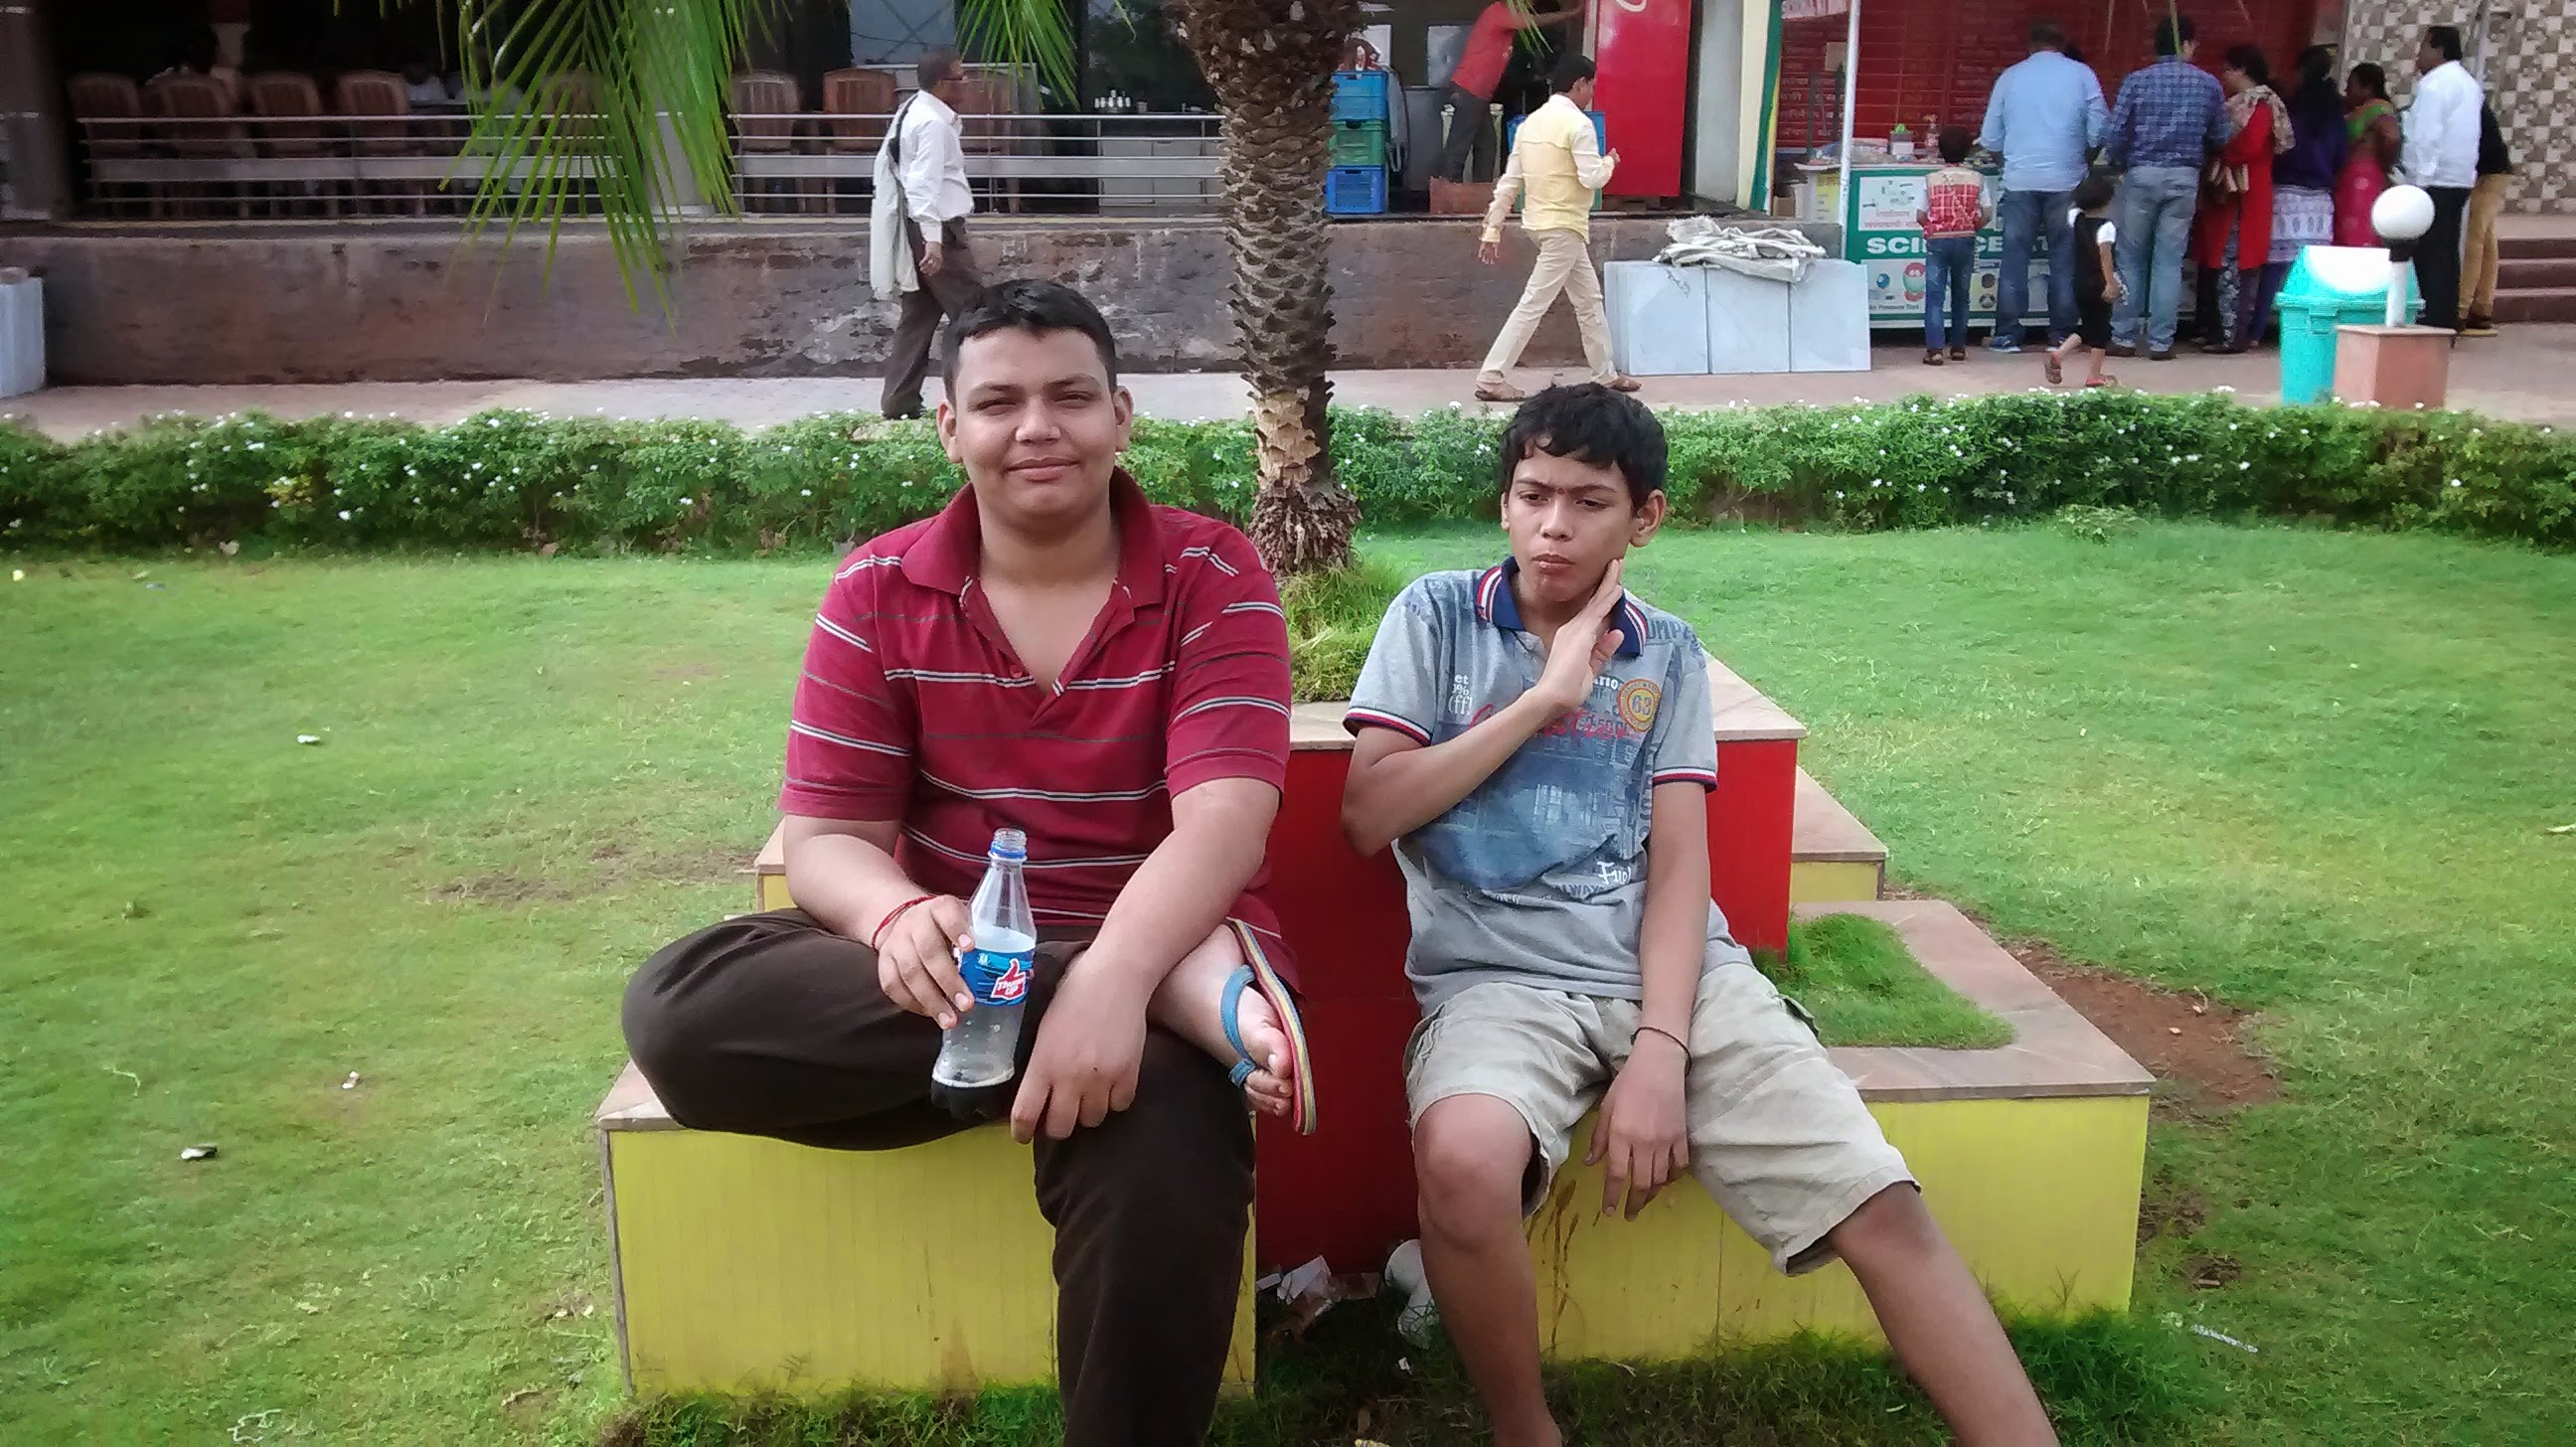
\includegraphics[width=1\textwidth]{running/1}
\end{figure}
\begin{figure}[H]

	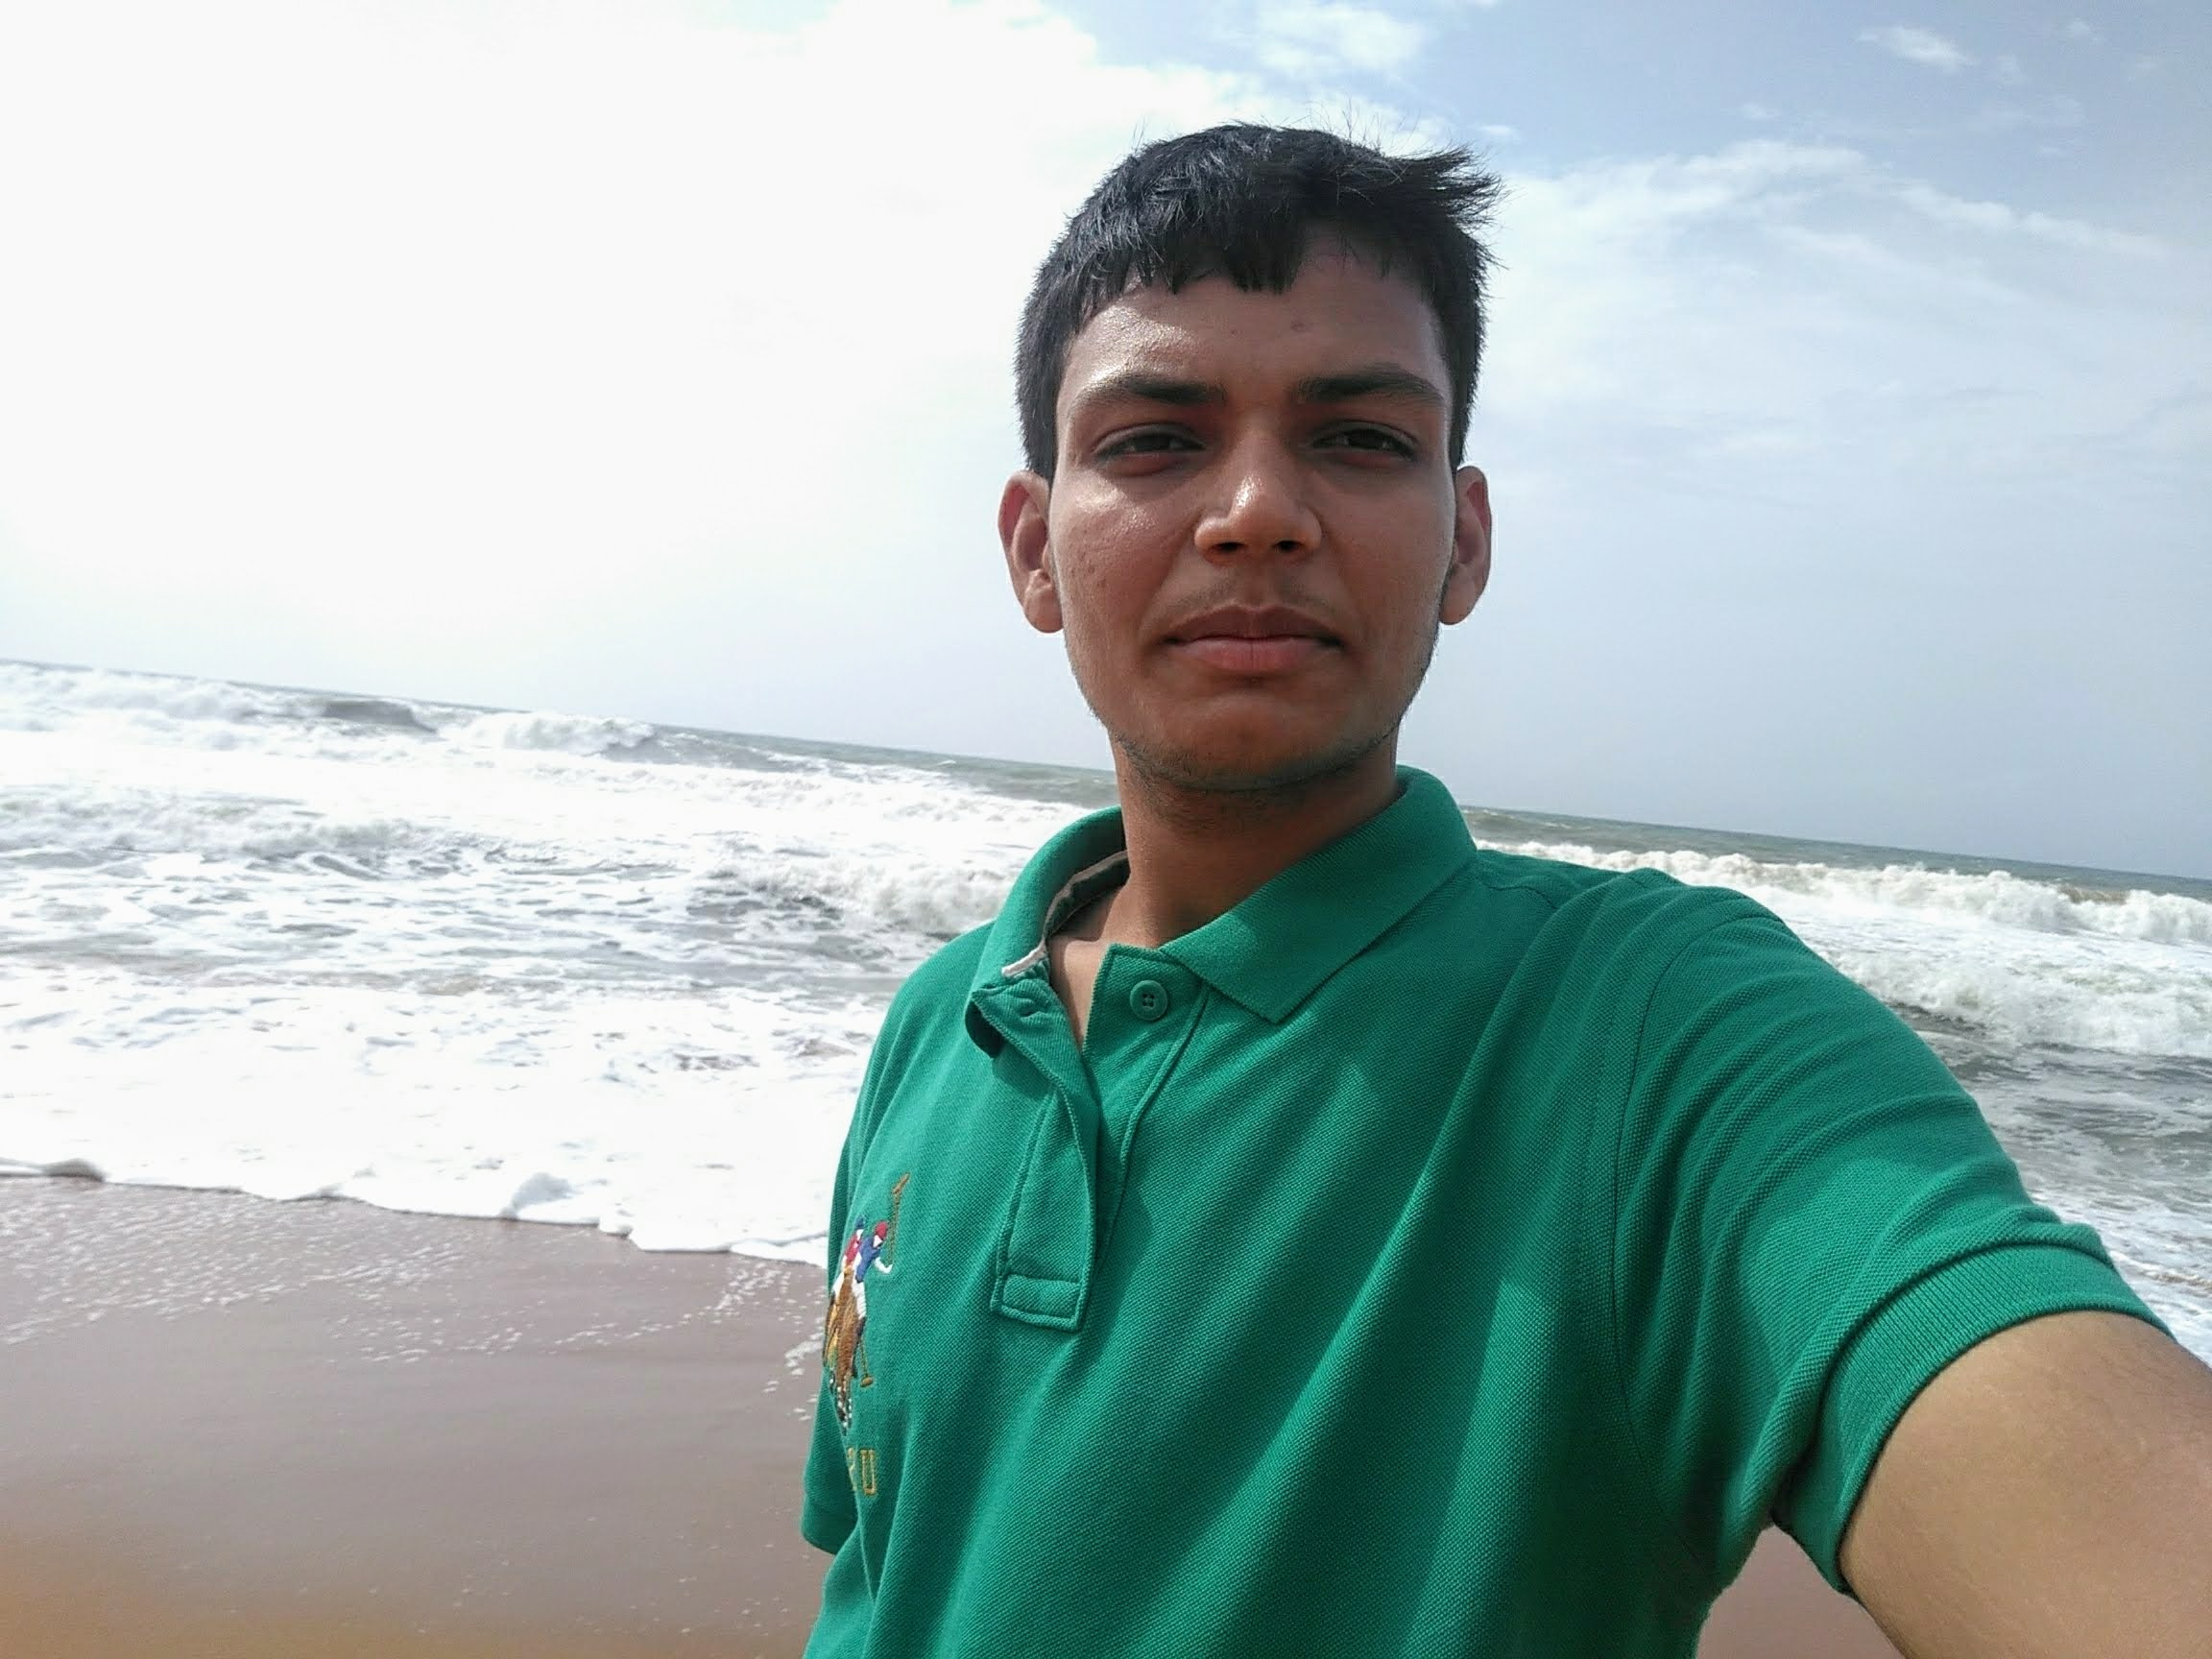
\includegraphics[width=1\textwidth]{running/2}
\end{figure}


\begin{figure}
	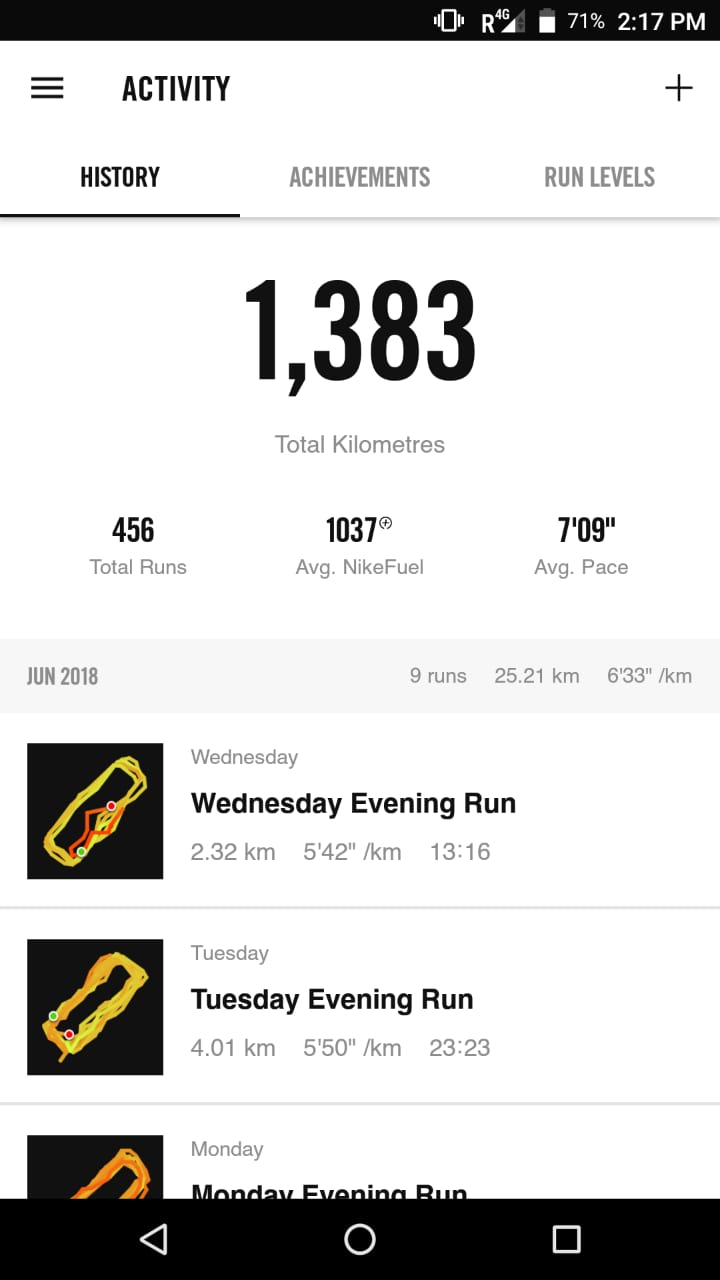
\includegraphics[width=0.8\textwidth]{running/1000}
\end{figure}



\begin{figure}

	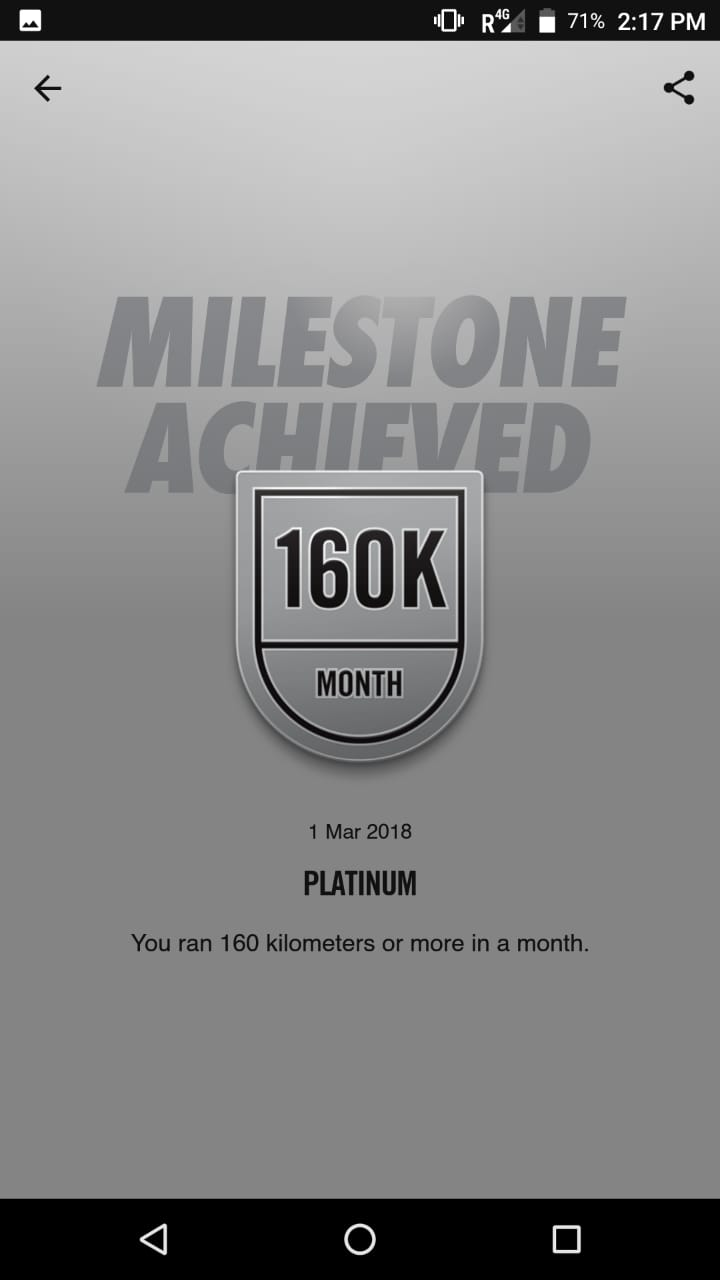
\includegraphics[width=0.8\textwidth]{running/160}
\end{figure}
\begin{figure}
	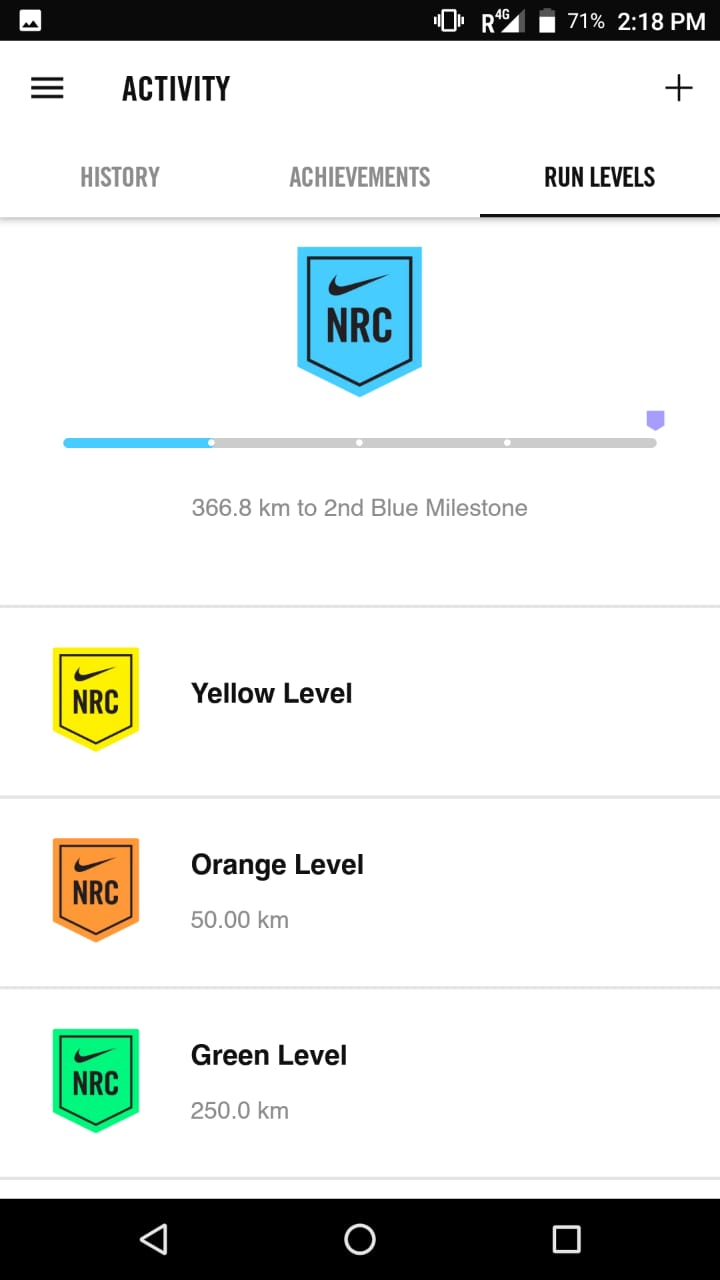
\includegraphics[width=0.8\textwidth]{running/blue}
\end{figure}


\end{document}